\documentclass{article}
\usepackage{graphicx}
\graphicspath{{./plots/}}
\begin{document}
\addtolength{\oddsidemargin}{-.875in}
\addtolength{\topmargin}{-.875in}
\begin{table}
\begin{tabular}{ |c|c|c| }
\hline
 Problem &   Function &       Derivative \\
\hline
1 & $f(x)=4 x^{5} + 5 x^{4}$&$ f'(x)=20 x^{4} + 20 x^{3}$\\
2 & $f(x)=e^{x} \sin{\left(x \right)}$&$ f'(x)=e^{x} \sin{\left(x \right)} + e^{x} \cos{\left(x \right)}$\\
3 & $f(x)=\frac{1}{x^{4} + 3 x}$&$ f'(x)=\frac{- 4 x^{3} - 3}{\left(x^{4} + 3 x\right)^{2}}$\\
4 & $f(x)=3 x^{2} \left(x^{3} + 1\right)^{7}$&$ f'(x)=63 x^{4} \left(x^{3} + 1\right)^{6} + 6 x \left(x^{3} + 1\right)^{7}$\\
5 & $f(x)=- 2 x^{2} + \cos^{4}{\left(x \right)}$&$ f'(x)=- 4 x - 4 \sin{\left(x \right)} \cos^{3}{\left(x \right)}$\\
6 & $f(x)=\frac{x}{x^{2} + 1}$&$ f'(x)=- \frac{2 x^{2}}{\left(x^{2} + 1\right)^{2}} + \frac{1}{x^{2} + 1}$\\
7 & $f(x)=\frac{x^{2} - 1}{x}$&$ f'(x)=2 - \frac{x^{2} - 1}{x^{2}}$\\
8 & $f(x)=\frac{3 x^{3}}{2}$&$ f'(x)=\frac{9 x^{2}}{2}$\\
9 & $f(x)=\log{\left(x e^{7 x} \right)}$&$ f'(x)=\frac{\left(7 x e^{7 x} + e^{7 x}\right) e^{- 7 x}}{x}$\\
10 & $f(x)=\frac{2 x^{4} + 3 x^{2} - 1}{x^{2}}$&$ f'(x)=\frac{8 x^{3} + 6 x}{x^{2}} - \frac{2 \cdot \left(2 x^{4} + 3 x^{2} - 1\right)}{x^{3}}$\\
11 & $f(x)=x^{3} \left(2 - x\right)^{0.2}$&$ f'(x)=- \frac{0.2 x^{3}}{\left(2 - x\right)^{0.8}} + 3 x^{2} \left(2 - x\right)^{0.2}$\\
12 & $f(x)=2 x - \frac{4}{\sqrt{x}}$&$ f'(x)=2 + \frac{2}{x^{\frac{3}{2}}}$\\
13 & $f(x)=\frac{4 \left(3 x - 1\right)^{2}}{7^{x} + x^{2}}$&$ f'(x)=\frac{4 \cdot \left(18 x - 6\right)}{7^{x} + x^{2}} + \frac{4 \left(3 x - 1\right)^{2} \left(- 7^{x} \log{\left(7 \right)} - 2 x\right)}{\left(7^{x} + x^{2}\right)^{2}}$\\
14 & $f(x)=\sqrt{x^{2} + 8}$&$ f'(x)=\frac{x}{\sqrt{x^{2} + 8}}$\\
15 & $f(x)=\frac{x}{\sqrt{1 - \log{\left(x \right)}^{2}}}$&$ f'(x)=\frac{1}{\sqrt{1 - \log{\left(x \right)}^{2}}} + \frac{\log{\left(x \right)}}{\left(1 - \log{\left(x \right)}^{2}\right)^{\frac{3}{2}}}$\\
16 & $f(x)=\frac{6}{\left(3 x^{2} - \pi\right)^{4}}$&$ f'(x)=- \frac{144 x}{\left(3 x^{2} - \pi\right)^{5}}$\\
17 & $f(x)=\frac{\left(3 x^{2} - \pi x\right)^{4}}{6}$&$ f'(x)=\frac{\left(24 x - 4 \pi\right) \left(3 x^{2} - \pi x\right)^{3}}{6}$\\
18 & $f(x)=\frac{x}{\left(\sqrt{3} \sqrt{x} + x^{2}\right)^{5}}$&$ f'(x)=\frac{x \left(- 10 x - \frac{5 \sqrt{3}}{2 \sqrt{x}}\right)}{\left(\sqrt{3} \sqrt{x} + x^{2}\right)^{6}} + \frac{1}{\left(\sqrt{3} \sqrt{x} + x^{2}\right)^{5}}$\\
19 & $f(x)=\left(x e^{x}\right)^{\pi}$&$ f'(x)=\frac{\pi \left(x e^{x}\right)^{\pi} \left(x e^{x} + e^{x}\right) e^{- x}}{x}$\\
20 & $f(x)=\operatorname{\arctan}^{10}{\left(2 x \right)}$&$ f'(x)=\frac{20 \operatorname{\arctan}^{9}{\left(2 x \right)}}{4 x^{2} + 1}$\\
21 & $f(x)=\left(e^{2 x} + e\right)^{0.5}$&$ f'(x)=\frac{1.0 e^{2 x}}{\left(e^{2 x} + e\right)^{0.5}}$\\
22 & $f(x)=\left(4 x + 7\right)^{3} \left(x^{6} + 1\right)^{5}$&$ f'(x)=30 x^{5} \left(4 x + 7\right)^{3} \left(x^{6} + 1\right)^{4} + 12 \left(4 x + 7\right)^{2} \left(x^{6} + 1\right)^{5}$\\
23 & $f(x)=\left(7 x + \sqrt{x^{2} + 3}\right)^{6}$&$ f'(x)=\left(7 x + \sqrt{x^{2} + 3}\right)^{5} \cdot \left(\frac{6 x}{\sqrt{x^{2} + 3}} + 42\right)$\\
24 & $f(x)=\frac{\frac{1}{x} + \frac{1}{x^{2}}}{x - 1}$&$ f'(x)=\frac{- \frac{1}{x^{2}} - \frac{2}{x^{3}}}{x - 1} - \frac{\frac{1}{x} + \frac{1}{x^{2}}}{\left(x - 1\right)^{2}}$\\
25 & $f(x)=x^{\frac{2}{3}} - \frac{1}{\sqrt[3]{x}}$&$ f'(x)=\frac{2}{3 \sqrt[3]{x}} + \frac{1}{3 x^{\frac{4}{3}}}$\\
26 & $f(x)=\left(\frac{2 x + 5}{7 x - 9}\right)^{0.5}$&$ f'(x)=\frac{\left(\frac{2 x + 5}{7 x - 9}\right)^{0.5} \cdot \left(7 x - 9\right) \left(- \frac{3.5 \cdot \left(2 x + 5\right)}{\left(7 x - 9\right)^{2}} + \frac{1.0}{7 x - 9}\right)}{2 x + 5}$\\
27 & $f(x)=\frac{\sin{\left(x \right)}}{\cos{\left(x \right)}}$&$ f'(x)=\frac{\sin^{2}{\left(x \right)}}{\cos^{2}{\left(x \right)}} + 1$\\
28 & $f(x)=\left(x^{2} + 3\right) \left(x^{3} + 4\right) e^{x}$&$ f'(x)=3 x^{2} \left(x^{2} + 3\right) e^{x} + 2 x \left(x^{3} + 4\right) e^{x} + \left(x^{2} + 3\right) \left(x^{3} + 4\right) e^{x}$\\
29 & $f(x)=\frac{5 x^{2} - 7 x}{x^{2} + 2}$&$ f'(x)=- \frac{2 x \left(5 x^{2} - 7 x\right)}{\left(x^{2} + 2\right)^{2}} + \frac{10 x - 7}{x^{2} + 2}$\\
30 & $f(x)=\log{\left(5 x^{2} + 9 \right)}^{3}$&$ f'(x)=\frac{30 x \log{\left(5 x^{2} + 9 \right)}^{2}}{5 x^{2} + 9}$\\
31 & $f(x)=\log{\left(5 x^{2} + 9 \right)}^{3}$&$ f'(x)=\frac{30 x \log{\left(5 x^{2} + 9 \right)}^{2}}{5 x^{2} + 9}$\\
32 & $f(x)=\cot{\left(6 x \right)}$&$ f'(x)=- 6 \cot^{2}{\left(6 x \right)} - 6$\\
33 & $f(x)=\tan{\left(x \right)} \sec^{2}{\left(x \right)}$&$ f'(x)=\left(\tan^{2}{\left(x \right)} + 1\right) \sec^{2}{\left(x \right)} + 2 \tan^{2}{\left(x \right)} \sec^{2}{\left(x \right)}$\\
34 & $f(x)=\operatorname{\arcsin}{\left(2^{x} \right)}$&$ f'(x)=\frac{2^{x} \log{\left(2 \right)}}{\sqrt{1 - 2^{2 x}}}$\\
35 & $f(x)=\tan{\left(\cos{\left(x \right)} \right)}$&$ f'(x)=- \left(\tan^{2}{\left(\cos{\left(x \right)} \right)} + 1\right) \sin{\left(x \right)}$\\
36 & $f(x)=\left(- x + \left(x^{2} - 1\right)^{5}\right)^{3}$&$ f'(x)=\left(- x + \left(x^{2} - 1\right)^{5}\right)^{2} \cdot \left(30 x \left(x^{2} - 1\right)^{4} - 3\right)$\\
37 & $f(x)=\sin{\left(3 x \right)} \sec{\left(x \right)}$&$ f'(x)=\sin{\left(3 x \right)} \tan{\left(x \right)} \sec{\left(x \right)} + 3 \cos{\left(3 x \right)} \sec{\left(x \right)}$\\
38 & $f(x)=\frac{\left(x - 1\right)^{3}}{x \left(x + 3\right)^{4}}$&$ f'(x)=- \frac{4 \left(x - 1\right)^{3}}{x \left(x + 3\right)^{5}} + \frac{3 \left(x - 1\right)^{2}}{x \left(x + 3\right)^{4}} - \frac{\left(x - 1\right)^{3}}{x^{2} \left(x + 3\right)^{4}}$\\
39 & $f(x)=\frac{\log{\left(3 x^{2} + 4 x \right)}}{\log{\left(5 \right)}}$&$ f'(x)=\frac{6 x + 4}{\left(3 x^{2} + 4 x\right) \log{\left(5 \right)}}$\\
40 & $f(x)=x e^{5 y} - 3 y$&$ f'(x)=\left[ - \frac{e^{5 y}}{5 x e^{5 y} - 3}\right]$\\
41 & $f(x)=x^{3} + x y + y^{2} - 7$&$ f'(x)=\left[ \frac{- 3 x^{2} - y}{x + 2 y}\right]$\\
42 & $f(x)=- 3 x + \frac{\sin{\left(y \right)}}{y^{2} + 1}$&$ f'(x)=\left[ \frac{3 y^{4} + 6 y^{2} + 3}{y^{2} \cos{\left(y \right)} - 2 y \sin{\left(y \right)} + \cos{\left(y \right)}}\right]$\\
\hline
\bottomrule
\end{tabular}
\end{table}
\begin{figure}
\caption{The plot for f(x)=$4 x^{5} + 5 x^{4}$ and its derivative f'(x)=$20 x^{4} + 20 x^{3}$}
\centering
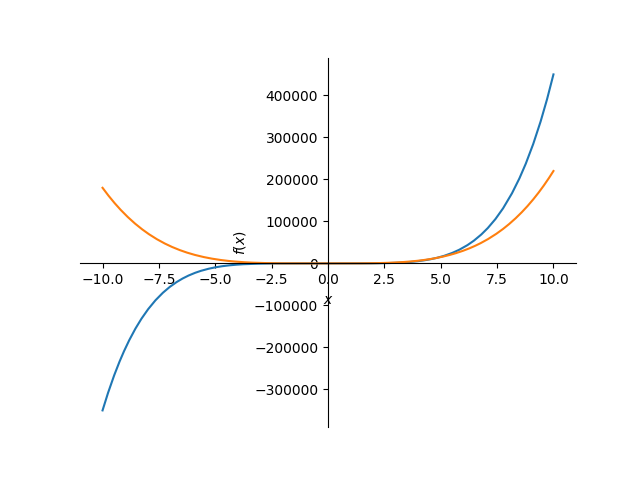
\includegraphics{plot_1}
\end{figure}\begin{figure}
\caption{The plot for f(x)=$e^{x} \sin{\left(x \right)}$ and its derivative f'(x)=$e^{x} \sin{\left(x \right)} + e^{x} \cos{\left(x \right)}$}
\centering
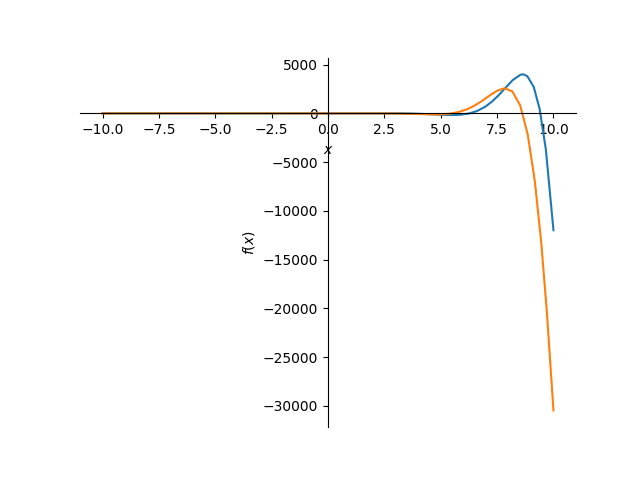
\includegraphics{plot_2}
\end{figure}\begin{figure}
\caption{The plot for f(x)=$\frac{1}{x^{4} + 3 x}$ and its derivative f'(x)=$\frac{- 4 x^{3} - 3}{\left(x^{4} + 3 x\right)^{2}}$}
\centering
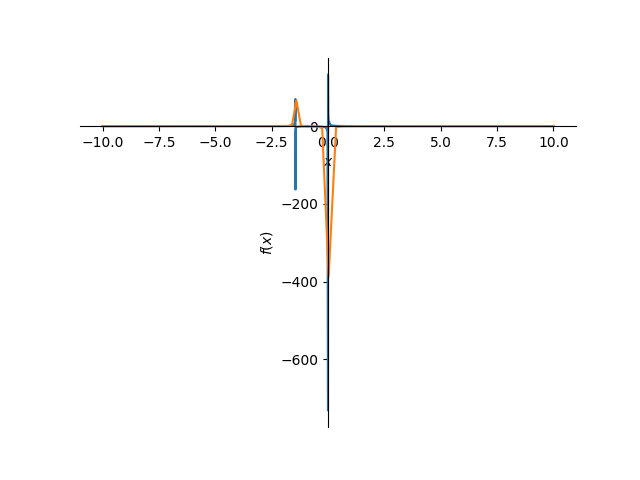
\includegraphics{plot_3}
\end{figure}\begin{figure}
\caption{The plot for f(x)=$3 x^{2} \left(x^{3} + 1\right)^{7}$ and its derivative f'(x)=$63 x^{4} \left(x^{3} + 1\right)^{6} + 6 x \left(x^{3} + 1\right)^{7}$}
\centering
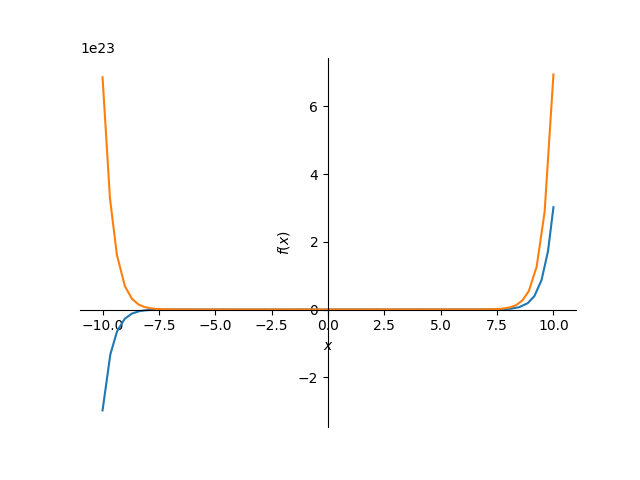
\includegraphics{plot_4}
\end{figure}\begin{figure}
\caption{The plot for f(x)=$- 2 x^{2} + \cos^{4}{\left(x \right)}$ and its derivative f'(x)=$- 4 x - 4 \sin{\left(x \right)} \cos^{3}{\left(x \right)}$}
\centering
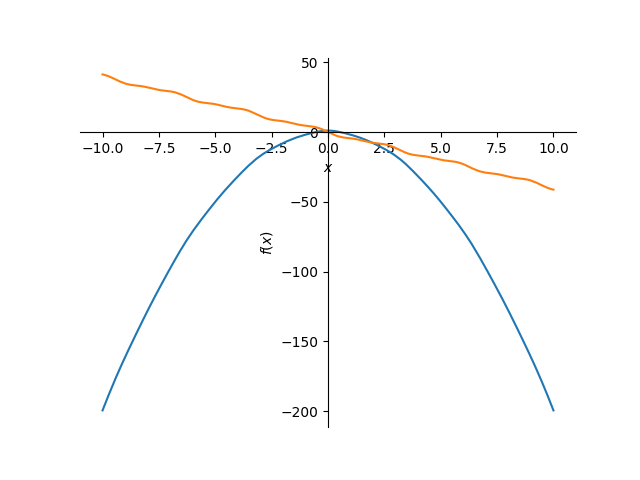
\includegraphics{plot_5}
\end{figure}\begin{figure}
\caption{The plot for f(x)=$\frac{x}{x^{2} + 1}$ and its derivative f'(x)=$- \frac{2 x^{2}}{\left(x^{2} + 1\right)^{2}} + \frac{1}{x^{2} + 1}$}
\centering
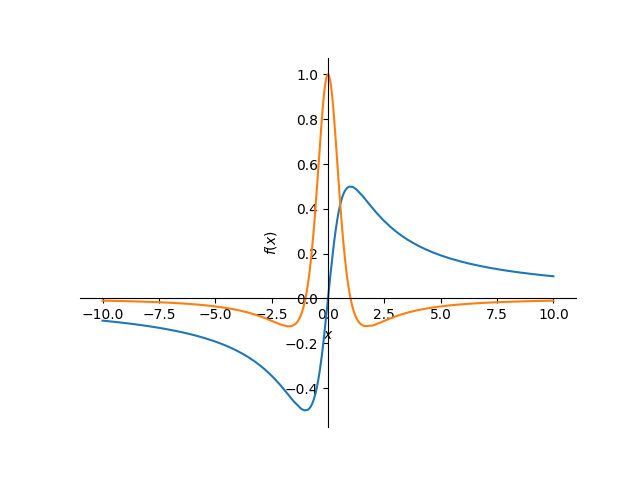
\includegraphics{plot_6}
\end{figure}\begin{figure}
\caption{The plot for f(x)=$\frac{x^{2} - 1}{x}$ and its derivative f'(x)=$2 - \frac{x^{2} - 1}{x^{2}}$}
\centering
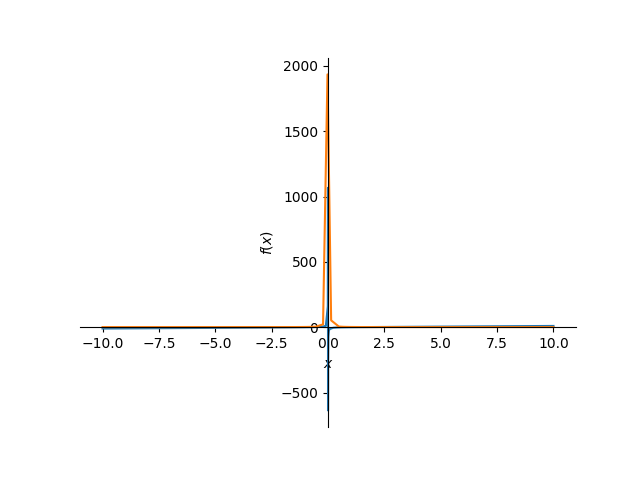
\includegraphics{plot_7}
\end{figure}\begin{figure}
\caption{The plot for f(x)=$\frac{3 x^{3}}{2}$ and its derivative f'(x)=$\frac{9 x^{2}}{2}$}
\centering
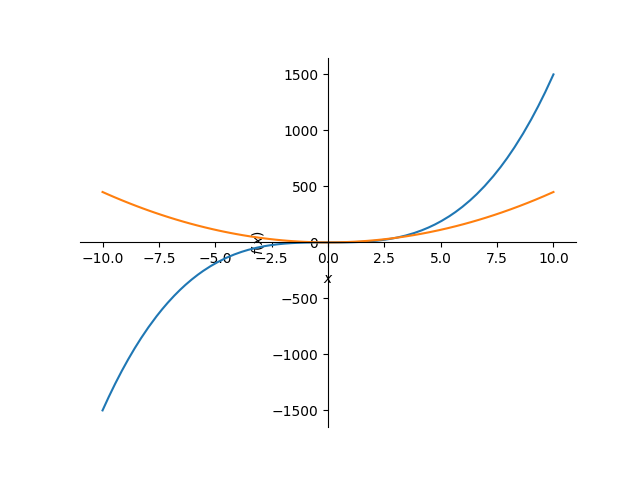
\includegraphics{plot_8}
\end{figure}\begin{figure}
\caption{The plot for f(x)=$\log{\left(x e^{7 x} \right)}$ and its derivative f'(x)=$\frac{\left(7 x e^{7 x} + e^{7 x}\right) e^{- 7 x}}{x}$}
\centering
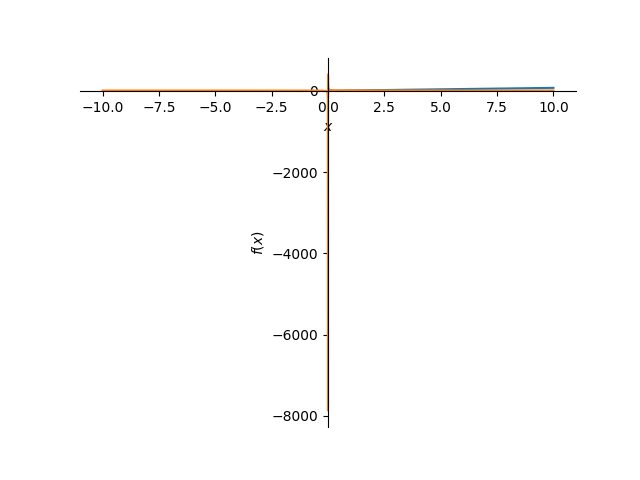
\includegraphics{plot_9}
\end{figure}\begin{figure}
\caption{The plot for f(x)=$\frac{2 x^{4} + 3 x^{2} - 1}{x^{2}}$ and its derivative f'(x)=$\frac{8 x^{3} + 6 x}{x^{2}} - \frac{2 \cdot \left(2 x^{4} + 3 x^{2} - 1\right)}{x^{3}}$}
\centering
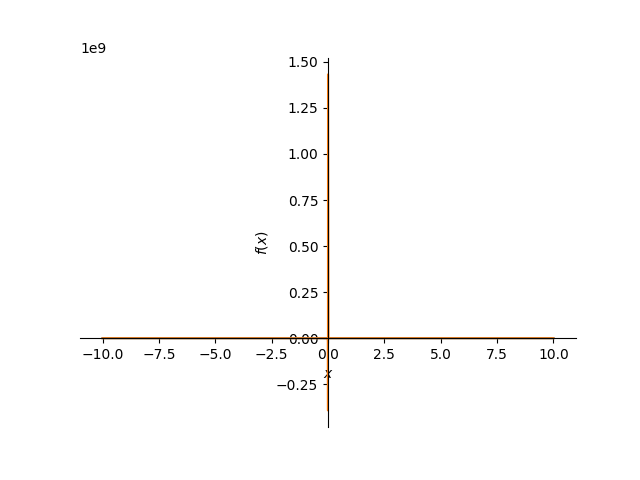
\includegraphics{plot_10}
\end{figure}\begin{figure}
\caption{The plot for f(x)=$x^{3} \left(2 - x\right)^{0.2}$ and its derivative f'(x)=$- \frac{0.2 x^{3}}{\left(2 - x\right)^{0.8}} + 3 x^{2} \left(2 - x\right)^{0.2}$}
\centering
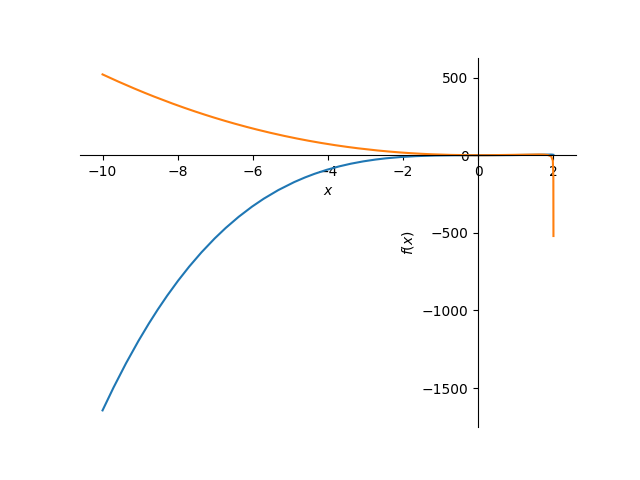
\includegraphics{plot_11}
\end{figure}\begin{figure}
\caption{The plot for f(x)=$2 x - \frac{4}{\sqrt{x}}$ and its derivative f'(x)=$2 + \frac{2}{x^{\frac{3}{2}}}$}
\centering
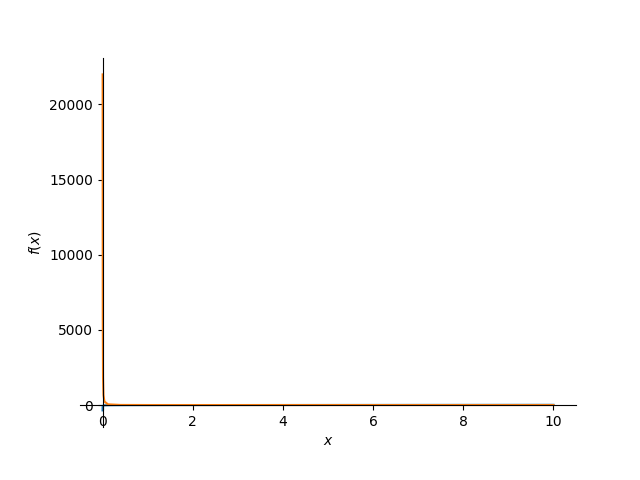
\includegraphics{plot_12}
\end{figure}\begin{figure}
\caption{The plot for f(x)=$\frac{4 \left(3 x - 1\right)^{2}}{7^{x} + x^{2}}$ and its derivative f'(x)=$\frac{4 \cdot \left(18 x - 6\right)}{7^{x} + x^{2}} + \frac{4 \left(3 x - 1\right)^{2} \left(- 7^{x} \log{\left(7 \right)} - 2 x\right)}{\left(7^{x} + x^{2}\right)^{2}}$}
\centering
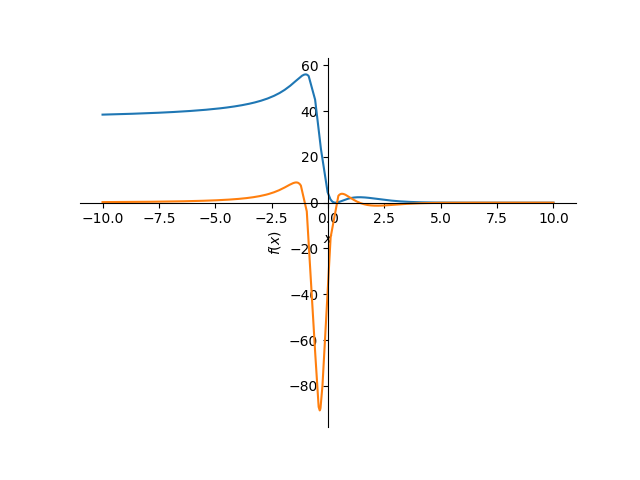
\includegraphics{plot_13}
\end{figure}\begin{figure}
\caption{The plot for f(x)=$\sqrt{x^{2} + 8}$ and its derivative f'(x)=$\frac{x}{\sqrt{x^{2} + 8}}$}
\centering
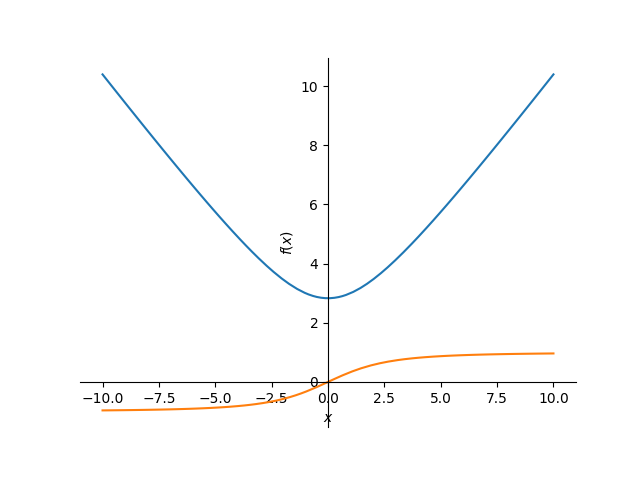
\includegraphics{plot_14}
\end{figure}\begin{figure}
\caption{The plot for f(x)=$\frac{x}{\sqrt{1 - \log{\left(x \right)}^{2}}}$ and its derivative f'(x)=$\frac{1}{\sqrt{1 - \log{\left(x \right)}^{2}}} + \frac{\log{\left(x \right)}}{\left(1 - \log{\left(x \right)}^{2}\right)^{\frac{3}{2}}}$}
\centering
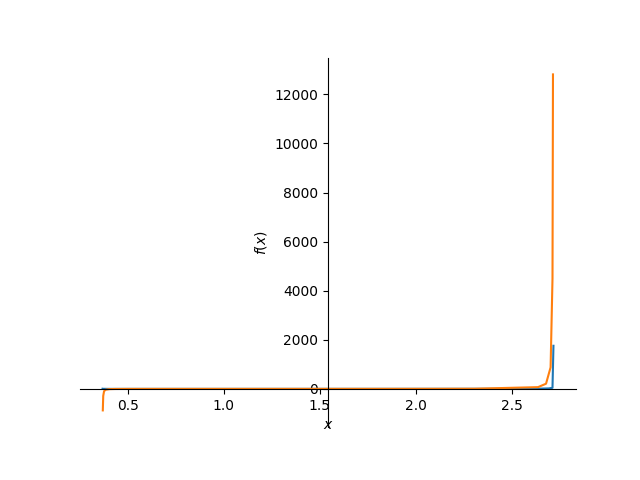
\includegraphics{plot_15}
\end{figure}\begin{figure}
\caption{The plot for f(x)=$\frac{6}{\left(3 x^{2} - \pi\right)^{4}}$ and its derivative f'(x)=$- \frac{144 x}{\left(3 x^{2} - \pi\right)^{5}}$}
\centering
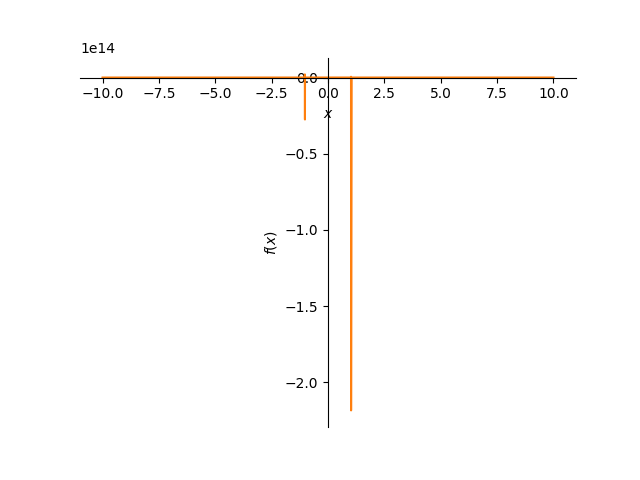
\includegraphics{plot_16}
\end{figure}\begin{figure}
\caption{The plot for f(x)=$\frac{\left(3 x^{2} - \pi x\right)^{4}}{6}$ and its derivative f'(x)=$\frac{\left(24 x - 4 \pi\right) \left(3 x^{2} - \pi x\right)^{3}}{6}$}
\centering
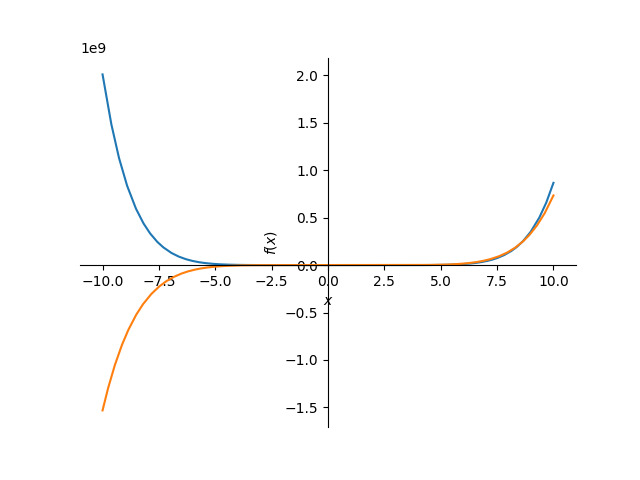
\includegraphics{plot_17}
\end{figure}\begin{figure}
\caption{The plot for f(x)=$\frac{x}{\left(\sqrt{3} \sqrt{x} + x^{2}\right)^{5}}$ and its derivative f'(x)=$\frac{x \left(- 10 x - \frac{5 \sqrt{3}}{2 \sqrt{x}}\right)}{\left(\sqrt{3} \sqrt{x} + x^{2}\right)^{6}} + \frac{1}{\left(\sqrt{3} \sqrt{x} + x^{2}\right)^{5}}$}
\centering
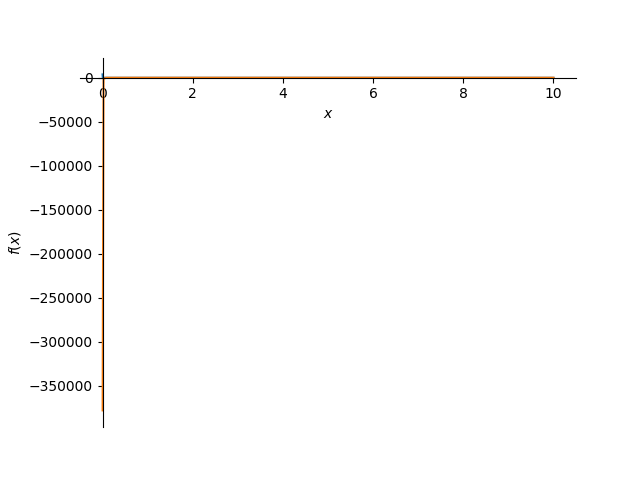
\includegraphics{plot_18}
\end{figure}\begin{figure}
\caption{The plot for f(x)=$\left(x e^{x}\right)^{\pi}$ and its derivative f'(x)=$\frac{\pi \left(x e^{x}\right)^{\pi} \left(x e^{x} + e^{x}\right) e^{- x}}{x}$}
\centering
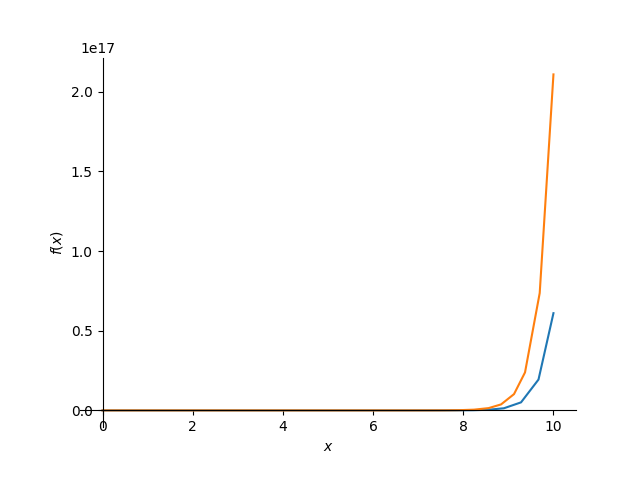
\includegraphics{plot_19}
\end{figure}\begin{figure}
\caption{The plot for f(x)=$\operatorname{\arctan}^{10}{\left(2 x \right)}$ and its derivative f'(x)=$\frac{20 \operatorname{\\arctan}^{9}{\left(2 x \right)}}{4 x^{2} + 1}$}
\centering
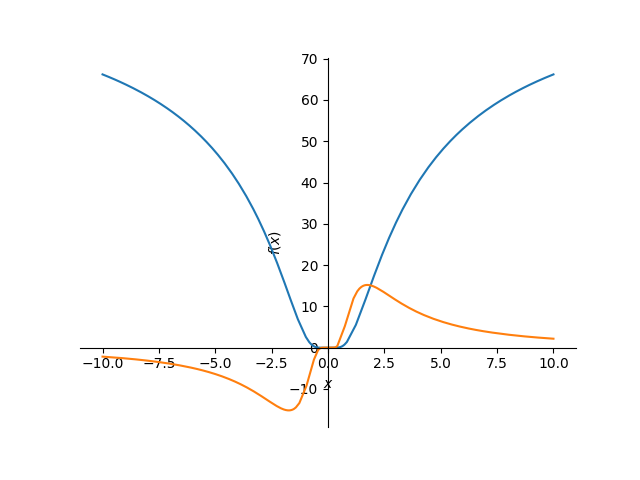
\includegraphics{plot_20}
\end{figure}\begin{figure}
\caption{The plot for f(x)=$\left(e^{2 x} + e\right)^{0.5}$ and its derivative f'(x)=$\frac{1.0 e^{2 x}}{\left(e^{2 x} + e\right)^{0.5}}$}
\centering
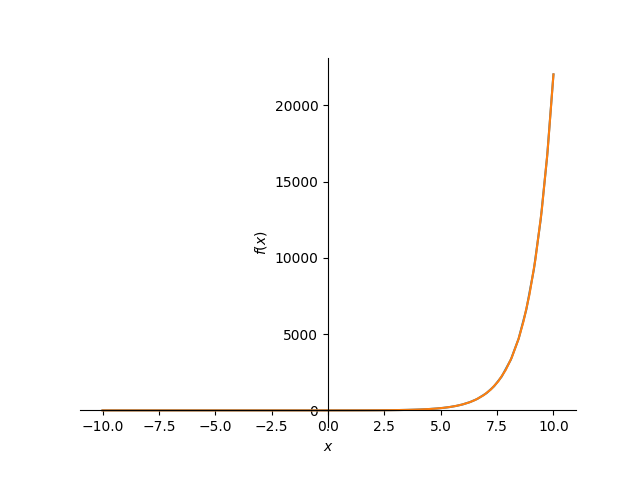
\includegraphics{plot_21}
\end{figure}\begin{figure}
\caption{The plot for f(x)=$\left(4 x + 7\right)^{3} \left(x^{6} + 1\right)^{5}$ and its derivative f'(x)=$30 x^{5} \left(4 x + 7\right)^{3} \left(x^{6} + 1\right)^{4} + 12 \left(4 x + 7\right)^{2} \left(x^{6} + 1\right)^{5}$}
\centering
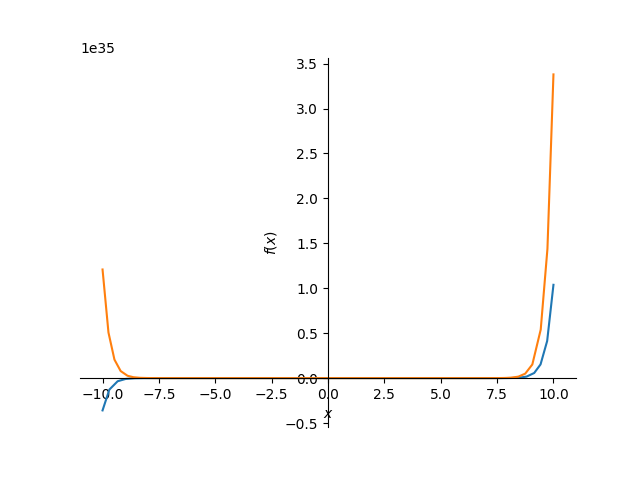
\includegraphics{plot_22}
\end{figure}\begin{figure}
\caption{The plot for f(x)=$\left(7 x + \sqrt{x^{2} + 3}\right)^{6}$ and its derivative f'(x)=$\left(7 x + \sqrt{x^{2} + 3}\right)^{5} \cdot \left(\frac{6 x}{\sqrt{x^{2} + 3}} + 42\right)$}
\centering
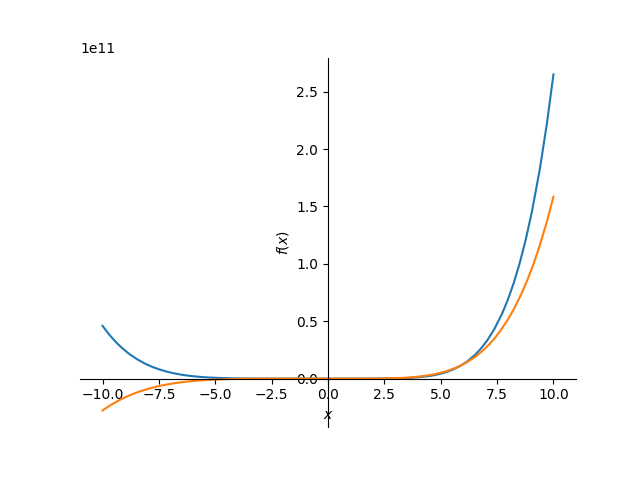
\includegraphics{plot_23}
\end{figure}\begin{figure}
\caption{The plot for f(x)=$\frac{\frac{1}{x} + \frac{1}{x^{2}}}{x - 1}$ and its derivative f'(x)=$\frac{- \frac{1}{x^{2}} - \frac{2}{x^{3}}}{x - 1} - \frac{\frac{1}{x} + \frac{1}{x^{2}}}{\left(x - 1\right)^{2}}$}
\centering
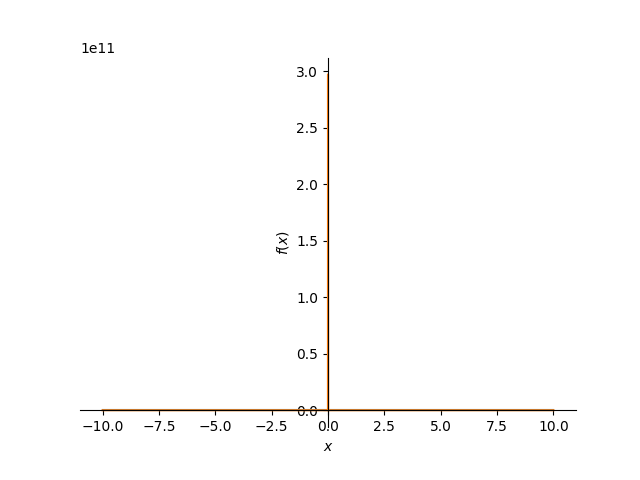
\includegraphics{plot_24}
\end{figure}\begin{figure}
\caption{The plot for f(x)=$x^{\frac{2}{3}} - \frac{1}{\sqrt[3]{x}}$ and its derivative f'(x)=$\frac{2}{3 \sqrt[3]{x}} + \frac{1}{3 x^{\frac{4}{3}}}$}
\centering
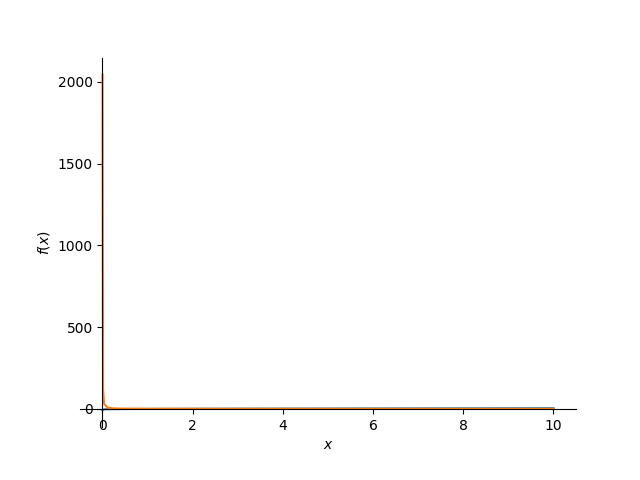
\includegraphics{plot_25}
\end{figure}\begin{figure}
\caption{The plot for f(x)=$\left(\frac{2 x + 5}{7 x - 9}\right)^{0.5}$ and its derivative f'(x)=$\frac{\left(\frac{2 x + 5}{7 x - 9}\right)^{0.5} \cdot \left(7 x - 9\right) \left(- \frac{3.5 \cdot \left(2 x + 5\right)}{\left(7 x - 9\right)^{2}} + \frac{1.0}{7 x - 9}\right)}{2 x + 5}$}
\centering
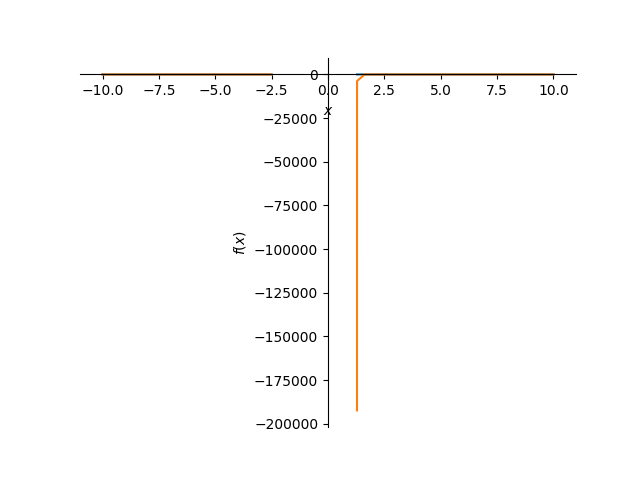
\includegraphics{plot_26}
\end{figure}\begin{figure}
\caption{The plot for f(x)=$\frac{\sin{\left(x \right)}}{\cos{\left(x \right)}}$ and its derivative f'(x)=$\frac{\sin^{2}{\left(x \right)}}{\cos^{2}{\left(x \right)}} + 1$}
\centering
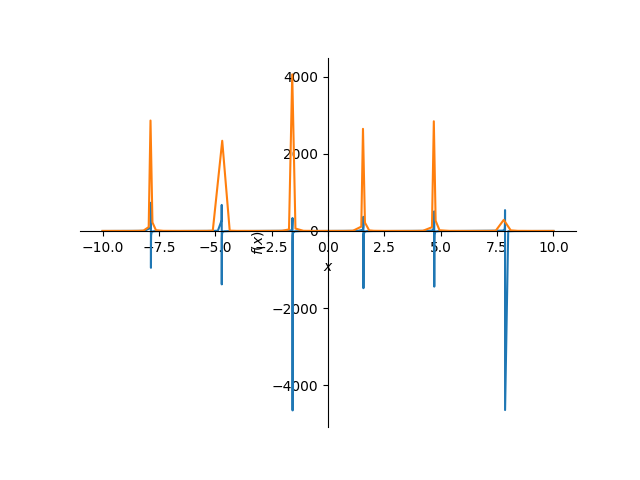
\includegraphics{plot_27}
\end{figure}\begin{figure}
\caption{The plot for f(x)=$\left(x^{2} + 3\right) \left(x^{3} + 4\right) e^{x}$ and its derivative f'(x)=$3 x^{2} \left(x^{2} + 3\right) e^{x} + 2 x \left(x^{3} + 4\right) e^{x} + \left(x^{2} + 3\right) \left(x^{3} + 4\right) e^{x}$}
\centering
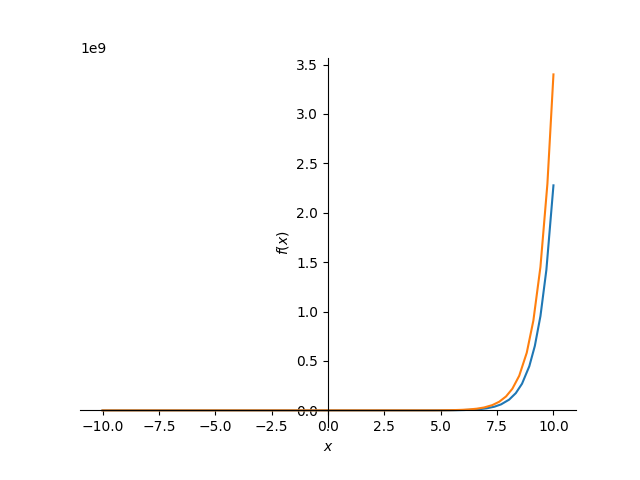
\includegraphics{plot_28}
\end{figure}\begin{figure}
\caption{The plot for f(x)=$\frac{5 x^{2} - 7 x}{x^{2} + 2}$ and its derivative f'(x)=$- \frac{2 x \left(5 x^{2} - 7 x\right)}{\left(x^{2} + 2\right)^{2}} + \frac{10 x - 7}{x^{2} + 2}$}
\centering
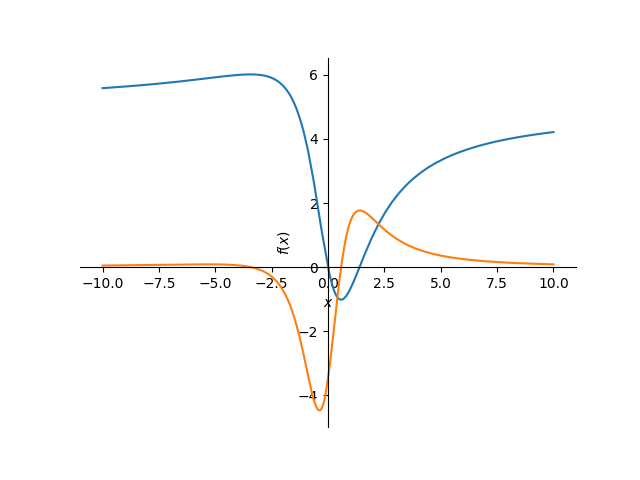
\includegraphics{plot_29}
\end{figure}\begin{figure}
\caption{The plot for f(x)=$\log{\left(5 x^{2} + 9 \right)}^{3}$ and its derivative f'(x)=$\frac{30 x \log{\left(5 x^{2} + 9 \right)}^{2}}{5 x^{2} + 9}$}
\centering
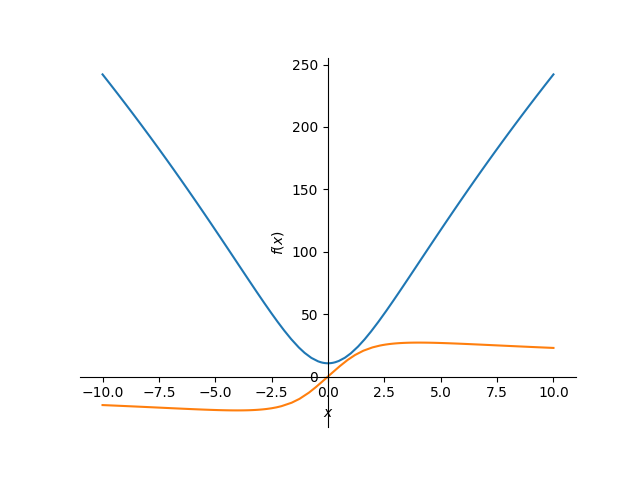
\includegraphics{plot_30}
\end{figure}\begin{figure}
\caption{The plot for f(x)=$\log{\left(5 x^{2} + 9 \right)}^{3}$ and its derivative f'(x)=$\frac{30 x \log{\left(5 x^{2} + 9 \right)}^{2}}{5 x^{2} + 9}$}
\centering
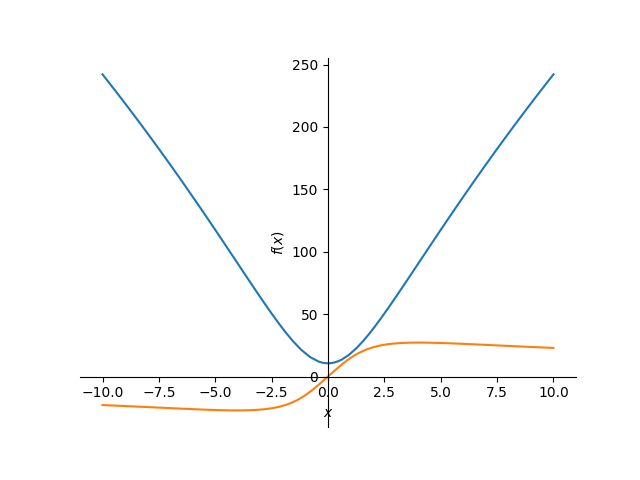
\includegraphics{plot_31}
\end{figure}\begin{figure}
\caption{The plot for f(x)=$\cot{\left(6 x \right)}$ and its derivative f'(x)=$- 6 \cot^{2}{\left(6 x \right)} - 6$}
\centering
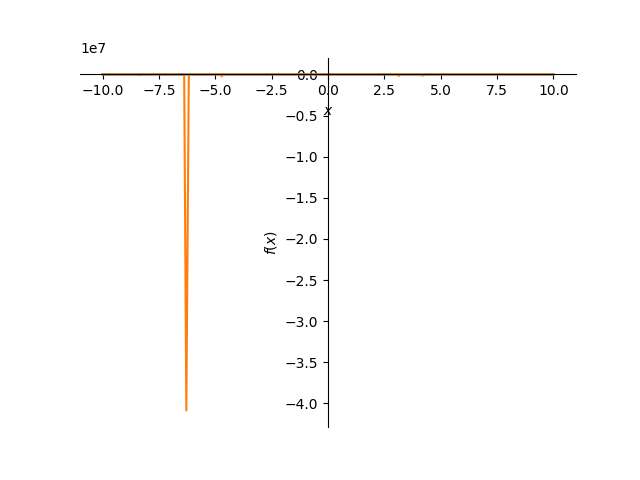
\includegraphics{plot_32}
\end{figure}\begin{figure}
\caption{The plot for f(x)=$\tan{\left(x \right)} \sec^{2}{\left(x \right)}$ and its derivative f'(x)=$\left(\tan^{2}{\left(x \right)} + 1\right) \sec^{2}{\left(x \right)} + 2 \tan^{2}{\left(x \right)} \sec^{2}{\left(x \right)}$}
\centering
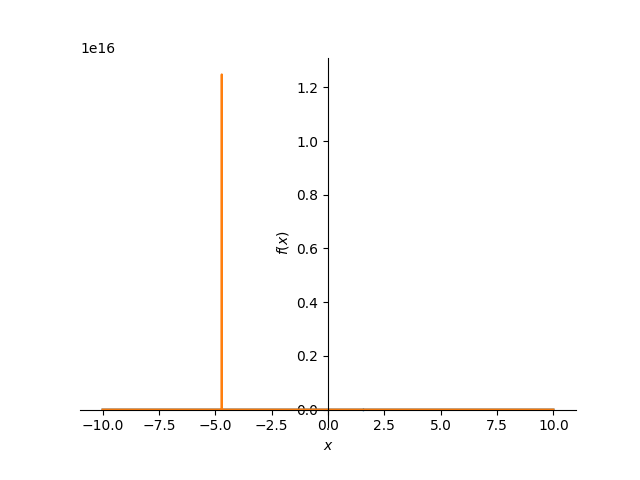
\includegraphics{plot_33}
\end{figure}\begin{figure}
\caption{The plot for f(x)=$\operatorname{\arcsin}{\left(2^{x} \right)}$ and its derivative f'(x)=$\frac{2^{x} \log{\left(2 \right)}}{\sqrt{1 - 2^{2 x}}}$}
\centering
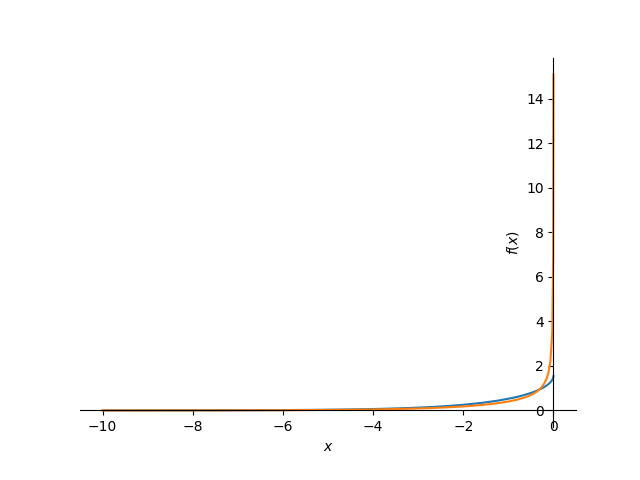
\includegraphics{plot_34}
\end{figure}\begin{figure}
\caption{The plot for f(x)=$\tan{\left(\cos{\left(x \right)} \right)}$ and its derivative f'(x)=$- \left(\tan^{2}{\left(\cos{\left(x \right)} \right)} + 1\right) \sin{\left(x \right)}$}
\centering
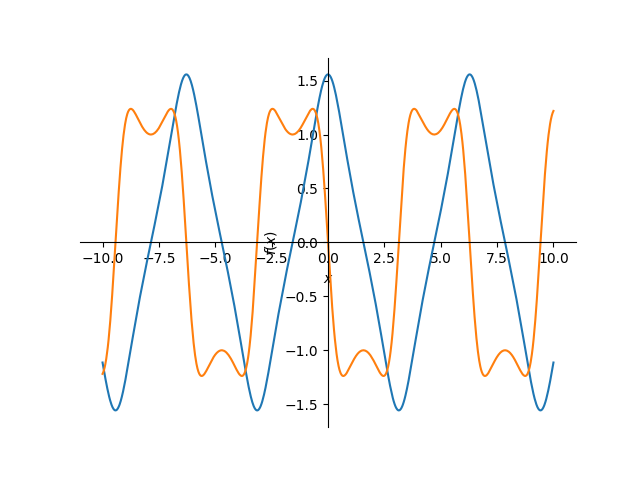
\includegraphics{plot_35}
\end{figure}\begin{figure}
\caption{The plot for f(x)=$\left(- x + \left(x^{2} - 1\right)^{5}\right)^{3}$ and its derivative f'(x)=$\left(- x + \left(x^{2} - 1\right)^{5}\right)^{2} \cdot \left(30 x \left(x^{2} - 1\right)^{4} - 3\right)$}
\centering
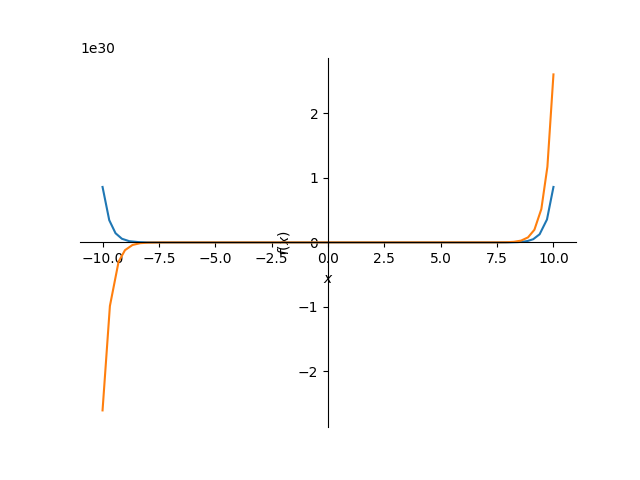
\includegraphics{plot_36}
\end{figure}\begin{figure}
\caption{The plot for f(x)=$\sin{\left(3 x \right)} \sec{\left(x \right)}$ and its derivative f'(x)=$\sin{\left(3 x \right)} \tan{\left(x \right)} \sec{\left(x \right)} + 3 \cos{\left(3 x \right)} \sec{\left(x \right)}$}
\centering
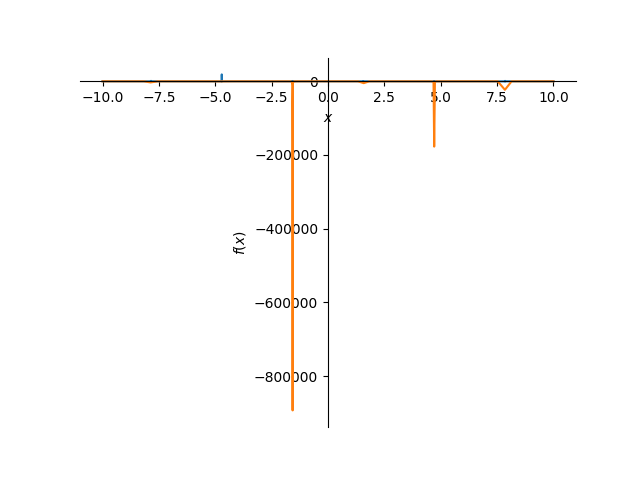
\includegraphics{plot_37}
\end{figure}\begin{figure}
\caption{The plot for f(x)=$\frac{\left(x - 1\right)^{3}}{x \left(x + 3\right)^{4}}$ and its derivative f'(x)=$- \frac{4 \left(x - 1\right)^{3}}{x \left(x + 3\right)^{5}} + \frac{3 \left(x - 1\right)^{2}}{x \left(x + 3\right)^{4}} - \frac{\left(x - 1\right)^{3}}{x^{2} \left(x + 3\right)^{4}}$}
\centering
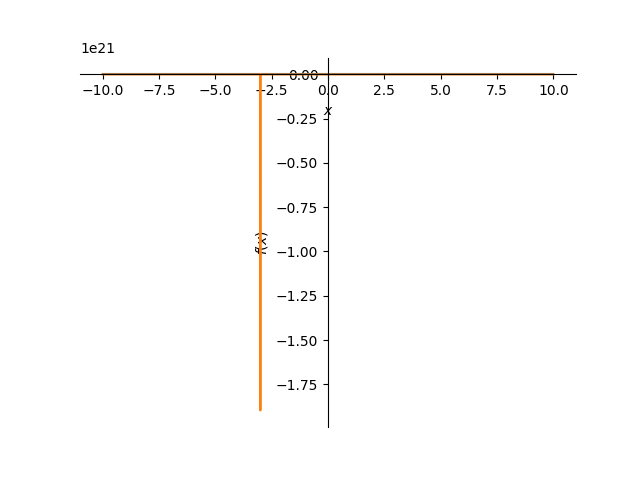
\includegraphics{plot_38}
\end{figure}\begin{figure}
\caption{The plot for f(x)=$\frac{\log{\left(3 x^{2} + 4 x \right)}}{\log{\left(5 \right)}}$ and its derivative f'(x)=$\frac{6 x + 4}{\left(3 x^{2} + 4 x\right) \log{\left(5 \right)}}$}
\centering
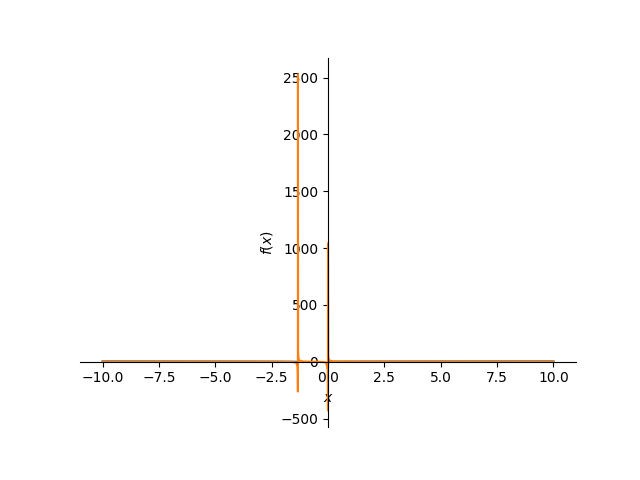
\includegraphics{plot_39}
\end{figure}